



%===============================================================================

% Matt Corsetti
% Dr. Tanzy Love
% PhD Defense 
% 18 August 2021



%===============================================================================

% Document class and mode setup

\documentclass{beamer}

\mode<presentation>{
    \usetheme{AnnArbor}
    \usecolortheme{wolverine}
}



%===============================================================================

% Defining custom colors

\definecolor{navyblue}{rgb}{0.0, 0.0, 0.5}
\definecolor{lightblue}{rgb}{0.9, 0.96, 1}
\definecolor{darkgreen}{rgb}{0, 0.5, 0}
\definecolor{darkpurple}{rgb}{0.44, 0.19, 0.63}


% Beamer theme options

\setbeamercolor{block title}{bg = navyblue, fg = white}
\setbeamercolor{block body}{bg = lightblue, fg = black}



%===============================================================================

% Packages

\usepackage{amsmath}
\usepackage{amssymb}
\usepackage{bm}
\usepackage[utf8]{inputenc}
\usepackage{pgf}
\usepackage{multirow}
\usepackage{qtree}
\usepackage{tikz}
\usepackage[normalem]{ulem}
    \useunder{\uline}{\ul}{}
\usepackage{xcolor}


\usetikzlibrary{arrows, automata}




%===============================================================================

% Title page setup

\title[Grafted and Vanishing Random Subspaces]{
Grafted and Vanishing Random Subspaces in Ensemble Classification
}

\author[T. Love]{
\texorpdfstring{\includegraphics[height=1.62cm,width=2cm]{Figures/UR_Logo.JPG} \\}{Lg}
\texorpdfstring{\smallskip}{Lg}
Tanzy Love and Matt Corsetti  
}

\institute[]{
Department of Biostatistics \\ and Computational Biology \\
University of Rochester
}

\date[October 18, 2024]{
October 18, 2024
}

\AtBeginSection[]
{
  \begin{frame}
    \frametitle{Table of Contents}
    \tableofcontents[currentsection]
  \end{frame}
}

\begin{document}
\maketitle

\addtobeamertemplate{frametitle}{}{
\begin{tikzpicture}[remember picture,overlay]
    \node[anchor = north east, yshift = 2pt] at (current page.north east) 
    {\includegraphics[height = 1.15cm]{Figures/UR_Logo3.JPG}};
\end{tikzpicture}}


%===============================================================================

\begin{frame}

    \frametitle{Overview}

    \underline{Overview}:
    \medskip
    
    \begin{itemize}
        \item Brief Overview of Ensemble Classification
            \begin{itemize}
                \item Tree learners
                \item Popular preexisting procedures
            \end{itemize}
            \medskip
        \item Grafted and Vanishing Random Subspaces
            \medskip
        \item Bagged Feature Weighted Random Forests
            \medskip
        \item Questions and Answers
    \end{itemize}
    
\end{frame}


%===============================================================================

\begin{frame}

    \frametitle{Classification and Regression Trees (CART)}
    
    \underline{Background}:
    
    \begin{columns}
        \begin{column}{0.6\textwidth}
            \begin{itemize}
                \item Proposed by Leo Breiman in 1984
                \item \textbf{Problem}: Linear regression models often 
                      perform poorly with complex real-world data
                \item \textbf{Idea}: Try fitting simple regression models to 
                      different partitions of the covariate space to achieve a 
                      better fit
                \item \textbf{Solution}: Partition up the covariate space using
                      a binary classification tree and fit a model to each 
                      subspace
            \end{itemize}
        \end{column}
        \begin{column}{0.4\textwidth}
            \begin{center}
                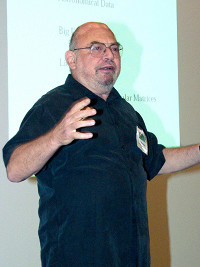
\includegraphics[width=0.75\textwidth]{Figures/Leo_Breiman.jpg}
            \end{center}
        \end{column}
    \end{columns}

\end{frame}


%===============================================================================

\begin{frame}

    \frametitle{Classification and Regression Trees (CART)}
    
    \underline{Growing a Regression Tree}:
    \bigskip
    
        \begin{itemize}
            \small
            \item The data consists of $p$ inputs and a response for each of $N$
                  observations, that is, $(x_i,y_i)$ for $i = 1,\dots, N$, with
                  $x_i = (x_{i1}, \dots, x_{ip})$
            \medskip
            \item The algorithm sequentially identifies a variable on which to 
                  make a split/partition as well as the respective split 
                  point/value
            \medskip
            \item CART partitions the covariate space into $M$ distinct,
                  non-overlapping regions $R_1, \dots, R_M$ and we model
                  the response as a constant $\gamma_m$ in each of the regions
                  as follows:
        %\end{itemize}
        \begin{equation}
            \small
            T(x) = \sum_{m=1}^M \gamma_m I(x \in R_m)
        \end{equation}
        \end{itemize}

\end{frame}


%===============================================================================

\begin{frame}

    \frametitle{Classification and Regression Trees (CART)}
    
    \underline{Boston Housing Data Example}:
    
    \begin{center}
        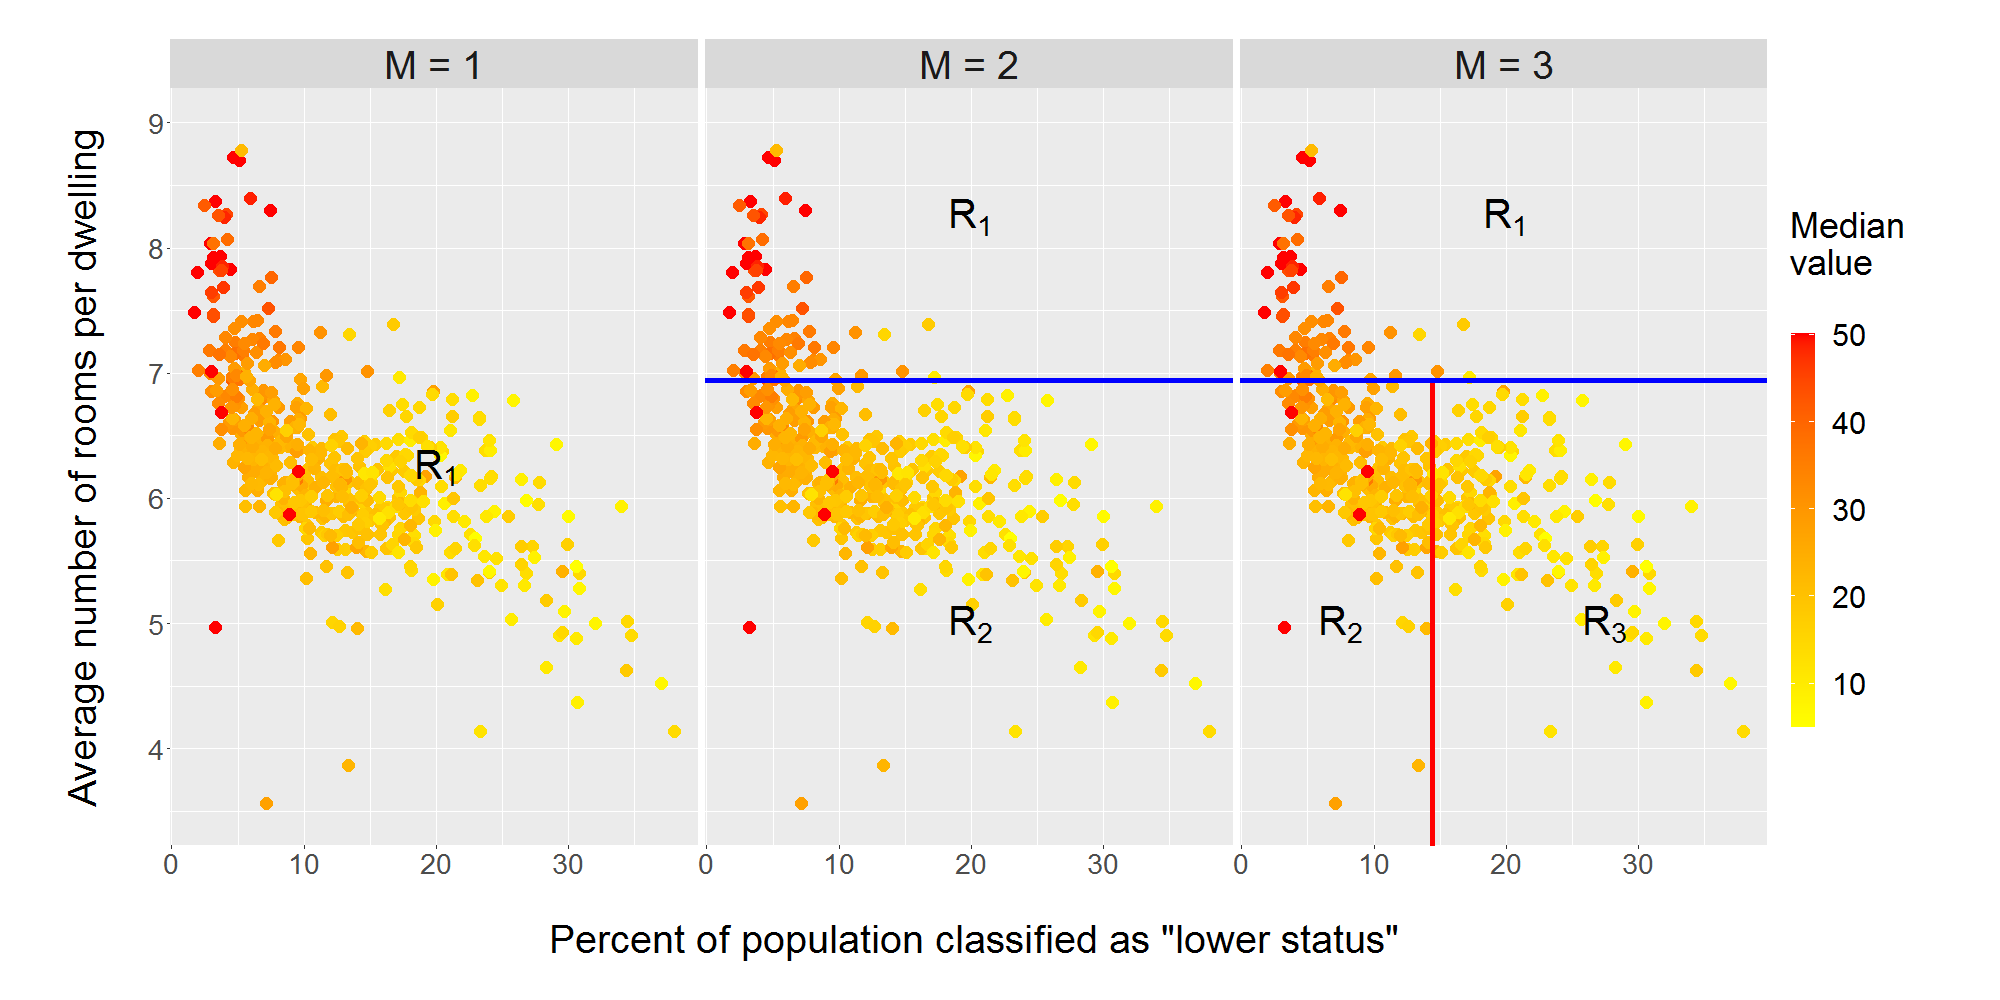
\includegraphics[width=\textwidth]{Figures/fig_boston_partitions.png}
    \end{center}
    
\end{frame}


%===============================================================================

\begin{frame}

    \frametitle{Classification and Regression Trees (CART)}
    
    \begin{columns}
    
    \begin{column}{0.5\textwidth}
        \begin{itemize}
            \footnotesize
            \item The first split $(\# \text{rooms} < 6.941)$ partitions the 
                  space into $R_1$ and $R_2$ 
            \item The second split $(\% \text{lower status})$ further divides up 
                  the $R_2$ subspace
        \end{itemize}
        \begin{center}
            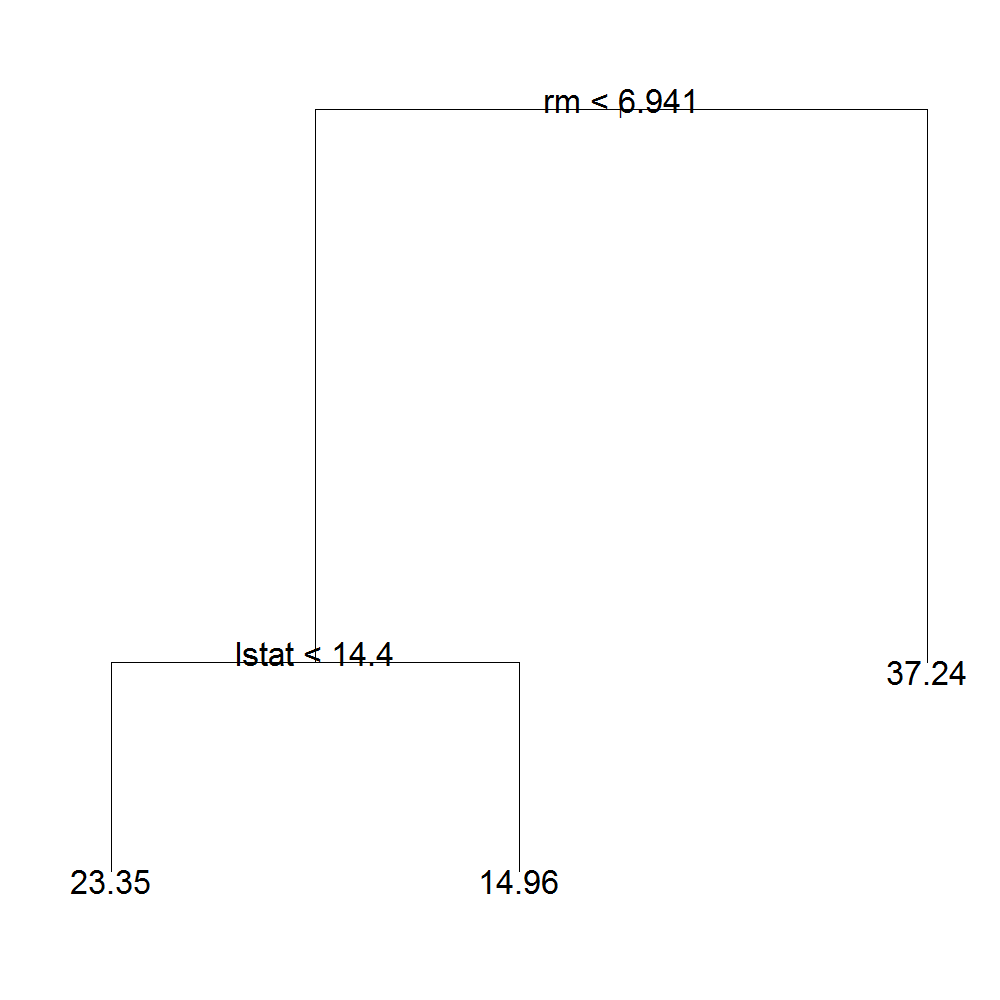
\includegraphics[width=0.8\textwidth]{Figures/fig_boston_cart_tree.png}
        \end{center}
   \end{column}
   
    \begin{column}{0.5\textwidth}
        \begin{itemize}
            \footnotesize
            \item The solution that minimizes the sum of squared errors uses the
              average of the $y_i$ in the region $R_m$ as the estimates for the
              $\gamma_m$'s
              \begin{equation*}
                \hat{\gamma}_m = \text{ave}(y_i|x_i \in R_M)
              \end{equation*}
        \end{itemize}
        \begin{center}
            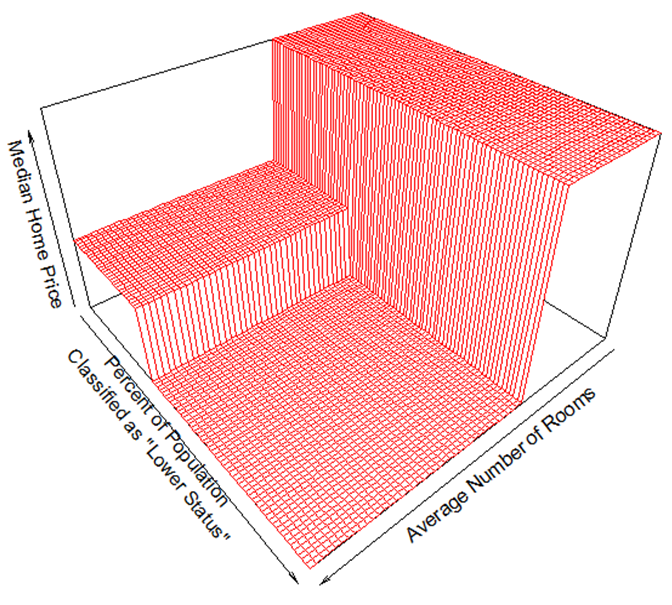
\includegraphics[width=0.8\textwidth]{Figures/fig_boston_skeleton_partitions.png}
        \end{center}
    \end{column}
    
    \end{columns}

\end{frame}


%===============================================================================

\begin{frame}

    \frametitle{Classification and Regression Trees (CART)}
    
    \footnotesize
    \underline{How do we pick the splits?}:
    \medskip

        \begin{itemize}
            \item Consider a split variable $k$ and value at which to split it $s$
                  and define the pair of half-planes
                  \begin{equation}
                    \underset{k,s}{\operatorname{min}} \Bigg[
                        \underset{\gamma_1}{\operatorname{min}}
                        \sum_{x_i \in R_1(k,s)} (y_i-\gamma_1)^2 +
                        \underset{\gamma_2}{\operatorname{min}}
                        \sum_{x_i \in R_2(k,s)} (y_i-\gamma_2)^2\Bigg]
                  \end{equation}
            \item Inner minimization is solved by 
                  $\hat{\gamma}_1 = \text{ave}(y_i|x_i \in R_1(k,s))$ and
                  $\hat{\gamma}_2 = \text{ave}(y_i|x_i \in R_2(k,s))$
            \item The partition is made on the best available split (greedy) 
                  identified using equation 2, then the process is repeated 
        \end{itemize}
        
%    \bigskip
%        
%    \underline{How/when do we stop?}: Cost-Complexity Pruning
%    
%    \begin{equation}
%        \sum_{m=1}^{|M|} \sum_{x_i \in R_m} (y_i - \hat{\gamma}_m)^2 + \alpha |M|
%    \end{equation}
        
\end{frame}


%===============================================================================

\begin{frame}

    \frametitle{Ensemble Methods}
    
    \begin{itemize}
        \item \textbf{Ensemble learning}: methods that join together ``simple" 
              models or ``weak" learners to form a committee or ensemble
        \medskip
        \item Ensembles leverage the combined strength of their base models
              to achieve increased predictive performance greater than that of
              the individual learners
        \medskip
        \item Generally speaking, ensembles are made stronger when there is
              disagreement and very little correlation among the learners
        \medskip
        \item ``Diversity and independence are important because the best 
           collective decisions are the product of disagreement and contest, not 
           consensus or compromise." -James Surowiecki, The Wisdom of Crowds
    \end{itemize}

\end{frame}


%===============================================================================

%===============================================================================

\begin{frame}

    \frametitle{Bootstrap Aggregation (Bagging)}
    
    \underline{Bagging}:
    \medskip
    
    \begin{itemize}
        \item Ensemble procedure that reduces variance in the estimate 
              $\hat{f}(x)$ by averaging over predictions from individual
              trees (reduces variance and leaves bias unchanged)
        \medskip
        \item Bagging with trees:
            \begin{itemize}
            \small
                \item Draw $B$ bootstrapped samples from the data 
                      $\boldsymbol{Z} = \{(x_1,y_1), \dots, (x_n,y_n)\}$
                \item For each bootstrap sample $\boldsymbol{Z}_{b}$, 
                      $b = 1,\dots,B$, fit a tree $T(x; \theta_b)$ and obtain
                      predictions, then average predictions across trees:
                \begin{equation}
                \footnotesize
                    \hat{f}_\text{Bagged}(x) = 
                    \frac{1}{B} \sum_{b=1}^B T(x; \theta_b),
                \end{equation}
                where $\theta_b$ characterizes the $b^\text{th}$ tree (split
                variables, cut points, terminal node values)
            \end{itemize}
    \end{itemize}

\end{frame}


%===============================================================================

\begin{frame}

    \frametitle{Random Subspaces}
    
    \underline{Random Subspaces}:
    \medskip
    
    \begin{itemize}
        \item Proposed by Tin Kam Ho in 1998, also known as ``attribute bagging"
        \medskip
        \item Random subspaces with trees:
        \begin{itemize}
            \small
            \item Draw $B$ randomly chosen subsets of the predictor variables
                  (referred to as ``feature subsets") from the data, each of size 
                  $r < p$
            \item For each feature subset $X^{b}_{\{n \times r\}}$ $b = 1,\dots,B$ 
                  fit a tree $T(x; \theta_b)$ and obtain the predictions, then
                  average predictions over trees:
            \begin{equation}
                \small
                    \hat{f}_\text{RSM}(x) = 
                    \frac{1}{B} \sum_{b=1}^B T(x; \theta_b)
                \end{equation}
        \end{itemize}
%        \item Building trees on different feature subsets can reduce correlation
%              between trees making for a stronger ensemble
    \end{itemize}

\end{frame}


%===============================================================================

\begin{frame}

    \frametitle{Random Forests}
    
%    \underline{Random Forests}:
%    \medskip
    
    \begin{itemize}
        \item Proposed by Leo Breiman in 2001, average over trees
        \item RF achieves this by randomly selecting $\text{mtry} \le p$ of the
              input variables as split candidates before each tree %split
        \item Improves the variance reduction of bagging by reducing correlation
              among trees in the ensemble
            \begin{itemize}
            \small
                \item Draw $B$ bootstrapped samples from the data 
                      $\boldsymbol{Z} = \{(x_1,c_1), \dots, (x_n,c_n)\}$
                \item For each bootstrap sample $\boldsymbol{Z}_{b}$, $b = 1,\dots,B$,
		\begin{itemize}
			\item select mtry of the variables  
                		\item fit a tree $T(x; \theta_b)$, with mtry candidate variables
			\item for predictions, choose the most popular class across trees:
		\end{itemize}
    	\end{itemize}
              \begin{equation}
                \small
                    \hat{f}_\text{RF}(x) = mode(T(x; \theta_{1:B}))
                    %\stackrel{mode}{B}
                \end{equation}
    \end{itemize}

\end{frame}


%===============================================================================

\begin{frame}

    \frametitle{Boosting}
    
    \underline{Boosting}:
    \medskip
    
    \begin{itemize}
        \small
        \item Propsed by Robert Schapire in 1990, sum of trees ensemble
        \item Fit tree $T(x, \theta_b)$ to residuals from ensemble consisting of 
              all trees that came before it (instead of $y$):
%              \begin{equation}
%                \small
%                \hat{\theta_b} =
%                    \underset{\theta_b}{\operatorname{argmin}}
%                    \Bigg[
%                        \sum_{i = 1}^n L(y_i, f_{b-1}(x_i) +
%                        T(x_i, \theta_b))
%                    \Bigg],
%              \end{equation}
        \item Fitting each tree to ensemble residuals allows ensemble
              to improve in areas where it performs poorly
        \item Boosted tree model is the sum over these trees
        \begin{equation}
            \hat{f}_\text{Boost}(x) = \sum_{b=1}^B T(x; \theta_b)
        \end{equation}
    \end{itemize}


\end{frame}


%===============================================================================

\begin{frame}

    \frametitle{Boosting}

    \begin{itemize}
        \item Shrunken version of new tree is added to the ensemble
              \begin{equation}
%                f_b(x) = f_{b-1}(x) + \omega T(x_i, \theta_b),
                f_\text{Boost}(x) = \sum_{b=1}^B \omega T(x; \theta_b)
                \quad 0 \le \omega \le 1
              \end{equation}
        \item Shrinkage prevents any one tree from being overly influential
        \medskip
        \item Shrinkage parameter $\omega$ controls rate at which
              boosting learns (smaller $\omega$ values with large forests sizes
              tend to work well)
    \end{itemize}


\end{frame}


%===============================================================================

\begin{frame}

    \frametitle{Combining Ensemble Methods}
    
    \begin{itemize}
        \item Much work has been done in combining data-partitioning methods 
              with feature-partitioning methods and also with boosting
    \end{itemize}
    
    \begin{center}
        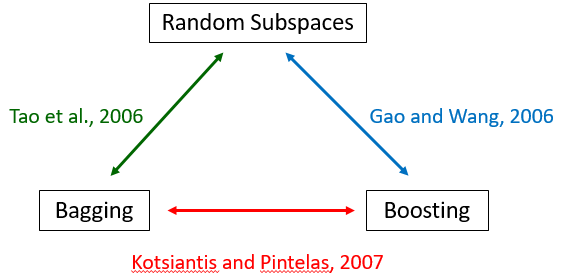
\includegraphics[width=0.6\textwidth]{Figures/Algorithm_Map.PNG}
    \end{center}
    
\end{frame}


%===============================================================================

\begin{frame}

    \frametitle{Overview}
    
    \underline{Overview}:
    \medskip
    
    \begin{itemize}
        \item \textcolor{lightgray} {Ensemble Classifiers}
            \begin{itemize}
                \item \textcolor{lightgray} {Tree learners}
                \item \textcolor{lightgray} {Popular preexisting procedures}
            \end{itemize}
            \medskip
        \item Grafted and Vanishing Random Subspaces
            \medskip
        \item \textcolor{lightgray} 
            {Bagged Feature Weighted Random Forests}
            \medskip
        \item \textcolor{lightgray} {Questions and answers}
    \end{itemize}
    
\end{frame}

%===============================================================================

\begin{frame}

    \frametitle{Motivating Statement}
    
    \underline{Problem}:
    \begin{itemize}
        \item Procedures that use random sampling of the input variables for
              split candidates (e.g. Random Forests, RSM) suffer when the \# 
              of truly informative features $s$ is small relative to $p$
        \item Feature (input variable) subsets are likely to contain many 
              non-informative features
        \item Learners built on these subsets can be harmful to ensemble
    \end{itemize}
    
    \medskip
    
    \underline{Solution}:
    \begin{itemize}
        \item Allow each tree to share information regarding variable importance
              in its feature subset with the trees that come after it in the 
              ensemble
    \end{itemize}
    
%    \medskip
%    
%    \textbf{Publication Status}: recently published
%        \textit{Pattern Analysis and Applications} 
    
    %\underline{Publication Status}:
    %\begin{itemize}
    %    \item In submission \textit{Pattern Analysis and Applications}
    %          (3rd round review)
    %\end{itemize}

\end{frame}


%===============================================================================

\begin{frame}

    \frametitle{Grafting and Vanishing Random Subspaces}
    
    \begin{columns}
    
    \begin{column}{0.75\textwidth}
    \small
        \underline{Grafting Random Subspaces (GRS)}:
        \medskip
        \begin{enumerate}
            \item Grow each tree on a bootstrapped sample and randomly chosen feature 
                subset of size $r<p$
            \item Identify most important variable in feature subset and 
                  recycle it across next $q$ subsets
        \end{enumerate}
        \medskip
        \underline{Main Idea}:
        \begin{itemize}
            \item Grafting allows new trees to reuse informative features 
            \item New trees explore how informative features
                interact with each other and features not yet
                randomly sampled
        \end{itemize}
        \end{column}
        
        \begin{column}{0.25\textwidth}
            \begin{center}
                \includegraphics[width=0.7\textwidth]{Figures/grafted.jpg}
            \end{center}
        \end{column}
    \end{columns}

\end{frame}


%===============================================================================

\begin{frame}

    \frametitle{Grafting and Vanishing Random Subspaces}
    
    \underline{Vanishing Random Subspaces (VRS)}:
    \medskip
    \begin{enumerate}
        \item Grow each tree on a bootstrapped sample and randomly chosen feature 
              subset of size $r<p$
        \item Identify least important variable in feature subset
        \item Temporarily exile feature from next $q$ subsets
    \end{enumerate}
    
    \bigskip
    
    \underline{Main Idea}:
    \begin{itemize}
        \item Exiling uninformative features creates a narrower but more enriched 
              pool of variable candidates
    \end{itemize}

\end{frame}


%===============================================================================

\begin{frame}

    \frametitle{Grafting and Vanishing Random Subspaces}
    
    \underline{Estimators}:
    \medskip
    \begin{itemize}
        \item Both GRS and VRS take the average over trees as the estimator
        \begin{equation}
            \hat{f}_\text{GRS/VRS}(x) = \frac{1}{B}\sum_{b=1}^B T(x; \theta_b)
        \end{equation}
        \item We also propose boosted versions of either algorithm (BoGRS and
              BoVRS) which are sum-of-shrunken-trees models
        \begin{equation}
            \hat{f}_\text{BoGRS/BoVRS} = \sum_{b=1}^B \omega T(x; \theta_b)
        \end{equation}
    \end{itemize}

\end{frame}


%===============================================================================

\begin{frame}

    \frametitle{Variable Importance}
    
    We consider grafting or vanishing either the most important or the least important variable.

\medskip

    Three measures of variable importance:
    
    \begin{enumerate}
        \item \textbf{First split} - variable used to split root node
        \item \textbf{Split frequency} - how often a variable is split on
        \item \textbf{Contribution to explained deviance}
    \end{enumerate}
    
\end{frame}


%%===============================================================================

\begin{frame}

    \frametitle{Variable Importance}
    
    \textbf{Contribution to explained deviance}
    
    \footnotesize
    
    \begin{itemize}
        \item Each non-terminal node has an associated deviance 
        \begin{equation*}
            D_v = \sum_{x_i \in R_v}(y_i - \hat{\gamma}_v)^2
        \end{equation*}
        where $v = 1, \dots, V$ indexes non-terminal nodes
        \item The gain in explained deviance from splitting a node is defined as
        \begin{equation*}
            \Delta = \frac{D_\text{parent}-(D_\text{left child} + D_\text{right child})}
                     {D_\text{root}}
        \end{equation*}
        \item Contribution to explained deviance for variable $j$ is the sum
              of the gains in explained deviance from non-terminal nodes that
              split on variable $j$
        \begin{equation*}
            \text{AggDev}_j = \sum_{v=1}^V \Delta_v 
                                I(\text{node } v \text{ splits on variable } j)
        \end{equation*}
    \end{itemize}

\end{frame}


%===============================================================================

\begin{frame}

    \frametitle{Variable Importance}
    
    \bigskip
    \underline{Optimal pairings}:

        \begin{enumerate}
            \item \textbf{VRS}: deviance + least important
            \medskip
            \item \textbf{VRS with boosting}: deviance + most important
            \medskip
            \item \textbf{GRS}: most commonly split + most important
            \medskip
            \item \textbf{GRS with boosting}: most commonly split + most important
            \medskip
        \end{enumerate}

\end{frame}


%===============================================================================
%
%\begin{frame}
%
%    \frametitle{The Grafting and Vanishing Parameter}
%    
%    \underline{Grafting/Vanishing Parameter $q$}:
%    \medskip
%    
%    \begin{itemize}
%        \item $q$ determines for how many successive feature subsets the 
%              variable is grafted or exiled
%        \begin{equation*}
%            q_b \sim \text{max}\{1, \text{Pois}(\sqrt{p}/2) \}
%        \end{equation*}
%        \item Draw $q_b$ after constructing the $b^\text{th}$ learner
%%        \bigskip
%%        \item Future work: 
%%        \begin{itemize}
%%            \item We'd like to make $q_b$ a function of both $p$ and $B$
%%                  (outside the scope of this paper)
%%        \end{itemize}
%    \end{itemize}
%
%\end{frame}
%
%
%%===============================================================================
%
%\begin{frame}
%
%    \frametitle{Simulation Design}
%    
%    We follow the simulation design of Hastie et al. 2017
%    \bigskip
%    
%    \underline{Simulation parameters}:
%    \medskip
%    \begin{itemize}
%        \item $n = 100$ (fixed number of observations)
%        \item $p = \{10,100,1000\}$ (number of predictor variables)
%        \item $s = \{5,50\}$ (sparsity level--number of truly informative variables)
%        \item $\rho = \{0.30,0.70\}$ (predictor autocorrelation level)
%        \item $\nu = \{0.05,0.42,2.07\}$ (signal-to-noise level)
%        \item 30 unique simulation settings
%    \end{itemize}
%
%\end{frame}
%
%
%%===============================================================================
%
%\begin{frame}
%
%    \frametitle{Simulation Design}
%    
%    \underline{Simulation data}:
%    \medskip
%    %\footnotesize
%    \small
%    \begin{enumerate}
%        \item $\beta_0$ = vector of true coefficients (first $s$ values are
%              sequence from 10 to 0.5)
%        \medskip
%        \item Predictor matrix $X \sim N_p(0,\Sigma)$ i.i.d. where $\Sigma$
%              has entry $(i,j)$ equal to $\rho^{|i-j|}$
%        \medskip
%        \item Response vector $y \sim N_n(X\beta_0, \sigma^2I)$, where 
%              $\sigma^2$ defined to meet desired SNR level, 
%              $\sigma^2 = \beta_0^T \Sigma \beta_0 / \nu$
%        \medskip
%        \item Acquire each ensemble's prediction error on validation set 
%              $(\tilde{X}, \tilde{y})$
%        \medskip
%        \item Repeat these steps 1,000 times and average prediction error 
%              across repeats
%    \end{enumerate}
%
%\end{frame}
%
%
%%===============================================================================

\begin{frame}

    \frametitle{Simulation Results}

    \begin{center}
        \includegraphics[width = \textwidth]
            {Figures/CART, p = 1000, s = 5, rho = 0.30, nu = 0.42.png}
    \end{center}

\end{frame}


%%===============================================================================
%
%\begin{frame}
%
%    \frametitle{Simulation Results}
%        \input{Tables/Table_GRSVRS_Simulation_Results}
%        
%    \begin{itemize}
%        \item At least one of our new procedures outperformed all preexisting 
%              ensemble competitors in 17 of the 30 simulation settings (7 by a
%              statistically significant margin)
%    \end{itemize}
%
%\end{frame}
%

%===============================================================================

\begin{frame}

    \frametitle{Experimental Design}
    
    \underline{Experimental Design - Data Analyses}:
    \medskip
    
    \begin{itemize}
        \small
        \item 200 individual experiments carried out on each of 12 real 
              datasets
        \item Training/test set split of 2/3:1/3 drawn at onset of each 
              experiment
        \item Ensemble predictive performances recorded at $B = {10}$ to 
              $B = 100$ trees in increments of 10
        \item MSE averaged across 200 individual experiments for each dataset
              and compared using paired T-tests
    \end{itemize}
    
    \bigskip
    
    \underline{Experimental Results}:
    \medskip
    
    \begin{itemize}
        \small
        \item New CART-based procedures outperformed preexisting ensembles in
              6 of the 12 datasets (4 by statistically significant margin)
    \end{itemize}

\end{frame}


%===============================================================================
%
%\begin{frame}
%
%    \frametitle{Experimental Results - Iranian Housing}
%    
%    \begin{figure}
%        \includegraphics[width = 0.875\textwidth]
%            {Figures/Iran_Performance_Plots.png}
%        \caption{Iranian Housing Performance Results $(n = 372, \ p = 103)$}
%    \end{figure}
%    
%
%\end{frame}
%
%
%===============================================================================

\begin{frame}

    \frametitle{Experimental Results - Gait Speed}
    
    \begin{figure}
        \includegraphics[width = .875\textwidth]
            {Figures/Gait_Performance_Plots.png}
        \caption{Gender Gait Speed Performance Results $(n = 48, \ p = 321)$}
    \end{figure}
    

\end{frame}


%===============================================================================

\begin{frame}

    \frametitle{Summary of Findings}

    \underline{Summary}:
    \medskip
    \begin{itemize}
        \item Grafting is better when there are few informative features ($\sim$5\%)
        \item Exiling tends to be better in situations with more informative 
              features ($\sim$50\%)
        \item For regression problems, we have boosted versions of GRS and VRS that tend to outperform their
              non-boosted counterparts
        \item Grafting tends to be the more promising of the two
\item What's best (but slower) is the Bayesian CART version of GRS and VRS
%        \item Future work: combine grafting and vanishing into one algorithm
    \end{itemize}

\end{frame}
%===============================================================================

\begin{frame}

    \frametitle{Postscript}

    \underline{If you'd like to look at the paper}:
    \medskip
    \begin{itemize}
        \item The Bayesian version of these methods uses BART fro forests of Bayesian trees
      \item GRS and VRS work even better in this case!
      \item Corsetti M. A. \&  Love T. M. (2022).
Grafted and Vanishing Random Subspaces.
Pattern Anal Appl. 25(1), 89-124.
    \end{itemize}

\end{frame}
    
%    
%%===============================================================================
%
%\begin{frame}
%
%    \frametitle{Overview}
%    
%    \underline{Overview}:
%    \medskip
%    
%    \begin{itemize}
%        \item \textcolor{lightgray} {Ensemble Methods}
%            \begin{itemize}
%                \item \textcolor{lightgray} {Tree learners}
%                \item \textcolor{lightgray} {Popular preexisting procedures}
%            \end{itemize}
%            \medskip
%        \item \textcolor{lightgray} {Grafted and Vanishing Random Subspaces}
%            \medskip
%        \item Bagged Feature Weighted Random Forests
%            \medskip
%        \item \textcolor{lightgray} {Questions and answers}
%    \end{itemize}
%    
%\end{frame}
%
%%===============================================================================
%
%\begin{frame}
%
%    \frametitle{Motivating Statement}
%    
%    \underline{Problem}: (similar motivating problem as GRS/VRS)
%    \begin{itemize}
%        \small
%        \smallskip
%        \item Random Forests suffers in settings where the number of truly
%              informative features $s$ is small relative to $p$
%        \item When drawing feature subsets to split the nodes, many 
%              uninformative features will be randomly selected
%        \item Sub-optimal solution: increase the mtry parameter to increase
%              chance of including valuable predictors--increases computational
%              burden
%    \end{itemize}
%    
%    \medskip
%    
%    \underline{Solution}:
%    \begin{itemize}
%        \small
%        \smallskip
%        \item Use weighted random sampling instead of simple random sampling
%              to draw feature subsets, with weights tilted in favor of
%              informative features
%        \item Establish weights in a pre-processing step before growing forest
%    \end{itemize}
%
%\end{frame}
%
%
%%===============================================================================
%
%\begin{frame}
%
%    \frametitle{Motivating Statement}
%    
%    \underline{Solution (continued)}:
%    \medskip
%
%    \begin{itemize}
%        \item Using weighted random sampling to select the feature subsets
%              for Random Forests is not a new idea:
%        \begin{itemize}
%            \item Enriched Random Forests (Amaratunga et al., 2008)
%            \item Feature-Weighted Random Forests (Ye et al. 2008)
%            \item Iterative Random Forests (Basu et al., 2018)
%        \end{itemize}
%        \medskip
%        \item \textbf{New Idea}: use ensemble methods (specifically bagging) to
%              establish better estimates of the feature weights in the 
%              pre-processing stage
%    \end{itemize}
%    
%    \bigskip
%    
%    \textbf{Publication Status}: In submission \textit{Machine Learning}
%    
%\end{frame}
%
%
%%===============================================================================
%
%\begin{frame}
%
%    \frametitle{Bagged Approach}
%    
%    \small{\underline{Bagged Approach}:}
%    \medskip
%
%    \begin{enumerate}
%    \footnotesize
%        \item Draw $Q$ bootstrapped samples from the training data
%        \item For each bootstrapped sample $\boldsymbol{Z}_q$, where 
%              $q = 1, \dots, Q$, apply the same feature-weighting algorithm 
%              (e.g. ReliefF) to the bootstrapped sample and extract the
%              $p$-vector of feature weights denoted $w_q$
%        \item Average over weight vectors to get ensemble estimate
%        \begin{equation}
%            \footnotesize
%            \hat{w}(x,y) = \frac{1}{Q} \sum_{q=1}^Q w_q(x,y)
%        \end{equation}
%        \item Construct the random forest using feature-weighted random 
%              sampling with the bagged ensemble-generated feature weights
%              $\hat{w}(x,y)$
%    \end{enumerate}
%    
%\end{frame}
%
%
%%===============================================================================
%
%\begin{frame}
%
%    \frametitle{ReliefF Feature Weights}
%    
%    \underline{ReliefF Algorithm} (Kononenko et al., 1997):
%    \medskip
%    \begin{itemize}
%        \small
%        \item An extension of the original Relief algorithm 
%              (Kira and Rendell, 1992) capable of handling missing data and 
%              multi-class problems
%        \item Key idea of all Relief-based algorithms: estimate a variable's
%              importance according to how well their values distinguish among
%              observations that are near each other
%        \item The algorithm should estimate the ability of attributes to separate 
%              each pair of classes regardless of which two classes are closest to each other
%        \item ReliefF searches for k near misses from each different class and 
%              averages their contributions for updating $W$, weighted with the 
%              prior probability of each class
%    \end{itemize}
%
%\end{frame}
%
%%
%%%===============================================================================
%%
%%\begin{frame}
%%
%%    \frametitle{Simulation Design}
%%    
%%    \underline{Simulation data}:
%%    \medskip
%%    
%%    \small
%%    \begin{itemize}
%%        \item We use the simulation model of Mease and Wyner (2008)
%%            \smallskip
%%        \item Probabilities of class membership for a binary response variable
%%              are generated using the model
%%            %
%%            \begin{equation}
%%                P(y = 1|x) = a + (1-2a) \cdot I
%%                \Bigg[
%%                    \sum_{j=1}^{s} x_j > s/2
%%                \Bigg].
%%            \end{equation}
%%            %
%%        \item Input features follow a multivariate uniform distribution, 
%%              $X \sim U[0,1]^p$
%%        \item Constant $a$ denotes the Bayes error rate such that 
%%            $0 \le a \le 1/2$
%%            \begin{itemize}
%%                \item Bayes error rate is the best possible error rate an 
%%                      estimator could achieve (oracle error rate)
%%            \end{itemize}
%%        \item Draw $n_\text{train} = 300$ and $n_\text{test} = 500$, 200 separate
%%              times for each combination of $a = \{0.1,0.2\}$, 
%%              $p = \{5,10,25,50,100,150\}$, and $s = 2$ and averaged the
%%              misclassification error rates
%%    \end{itemize}
%%
%%\end{frame}
%%
%%
%%%===============================================================================
%%
%%\begin{frame}
%%
%%    \frametitle{Simulation Results}
%%
%%    \begin{center}
%%        \includegraphics[width = 0.85\textwidth]
%%            {Figures/Mease_Results.png}
%%    \end{center}
%%
%%\end{frame}
%%
%
%%===============================================================================
%
%\begin{frame}
%
%    \frametitle{Experimental Design}
%    
%    \underline{Experimental Design}:
%    \medskip
%    
%    \begin{itemize}
%        \item 200 individual experiments carried out on 12 real datasets
%        \item Training/testing split of 25\%:75\% drawn at onset of each 
%              experiment
%        \item Average misclassification error rate trajectories recorded at 
%              ensemble sizes ranging from $B = 10$ through $B = 200$
%    \end{itemize}
%
%\end{frame}
%
%
%%===============================================================================
%
%\begin{frame}
%
%    \frametitle{Experimental Design}
%    
%    \input{Tables/Table_BRWRF_real_data_summary}
%
%\end{frame}
%
%
%%===============================================================================
%
%
%\begin{frame}
%
%    \frametitle{Experimental Results}
%    
%    \begin{center}
%        \includegraphics[width = \textwidth]
%            {Figures/brwrf_real_data_1.png}
%    \end{center}
%
%\end{frame}
%
%
%%===============================================================================
%
%\begin{frame}
%
%    \frametitle{Experimental Results}
%    
%    \begin{center}
%        \includegraphics[width = \textwidth]
%            {Figures/brwrf_real_data_2.png}
%    \end{center}
%
%\end{frame}
%
%
%%===============================================================================
%
%\begin{frame}
%
%    \frametitle{Experimental Results}
%    
%    \underline{Experimental Results}:
%    \medskip
%    \begin{itemize}
%        \item BRWRF was the best performer on 8 of the 12 datasets (7 by 
%              statistically significant amounts)
%        \item Key performance pattern occurs in 7 of the 12 datasets
%            \begin{itemize}
%                \item Traditional Random Forests outperforms ReliefF Weighted
%                      Random Forests
%                \item Bagged ReliefF Weighted Random Forests outperforms 
%                      traditional Random Forests
%                \item Demonstrates the need for better methods to estimate
%                      feature weights
%            \end{itemize}
%    \end{itemize}
%
%\end{frame}
%
%
%%===============================================================================

\begin{frame}

    \frametitle{Acknowledgements}
    
   
    \begin{itemize}
\item Matt Corsetti now works for Travelers Insurance (remotely from Rochester)
        \item His work was supported by our T32 Training Grant in Environmental Health Biostatistics (T32ES007271)
    \end{itemize}

\end{frame}


%===============================================================================

\begin{frame}

    \frametitle{References}
    
    \scriptsize
    \begin{enumerate}
        \item Breiman, L., Friedman, J. H., Olshen, R. A., \& Stone, C. J. 
              (1984). Classification and regression trees. 
              Boca Raton, FL: CRC Press.
        \item Ho, T. K. (1995). Random Decision Forests.
              Proceedings of the 3rd International Conference on Document 
              Analysis and Recognition, 278-282.
        \item Hastie, T., Tibshirani, R., \& Friedman, J. H. (2004). 
              The elements of statistical learning: Data mining, inference, and 
              prediction: With 200 full-color illustrations. 
              New York: Springer.
        \item Schapire, R. E. (1990). The strength of weak learnability.
              Machine Learning, 5(2), 197-227.
	\item Corsetti M. A. \&  Love T. M. (2022).
Grafted and Vanishing Random Subspaces.
Pattern Anal Appl. 25(1), 89-124.
    \end{enumerate}
    
\end{frame}


%===============================================================================

\begin{frame}

    \frametitle{Questions and Answers}

    \begin{center}
        \huge
        Thank you
    \end{center}

\end{frame}



\end{document}
